\section[Prerequisites]{Prerequisites}

LPUS has some prerequisites for the environment running on. Before moving on to
the LPUS system, we will briefly go through each prerequisite and explain why.

\subsection[Operating system]{Operating system}

Windows machine running LPUS must be 7 or above. While the Windows server is
not tested, the Windows home machine with version 7 or above is guaranteed to
execute LPUS without any problem.  The reason why LPUS does not support Windows
XP and the lower Windows version is that the third parties that LPUS depends
on. Third-parties used by LPUS deprecate the old Windows version by using newer
Windows API. Although we can rewrite the module to use the old Windows API
which will work on more Windows version, the work burden would be too much.

\subsection[Requirements for the driver]{Requirements for the driver}

The LPUS kernel-mode driver must be signed or \textit{test mode} is on.  In
Section 2.3.1, we discussed how Windows enforces driver signing to protect
untrusted drivers from loading into the system. Thus, the LPUS kernel driver
must be signed if we want to load in the system. In this thesis, we want to
demonstrate LPUS's usability, which is why signing the driver is not needed,
and instead, we use a development environment for testing the driver. This test
environment is called test mode, a feature which allows loading unsigned
driver. To enable the environment, one must enter \texttt{bcdedit /set
testsigning on} on an elevated command prompt and reboot the machine. On
rebooting, a small text read \texttt{Test Mode} will be visible in the bottom
right corner on the Desktop as in Figure \ref{fig:testmode}.

\begin{figure}[h]
  \centering
  \caption{Testmode enabled}
  \label{fig:testmode}
  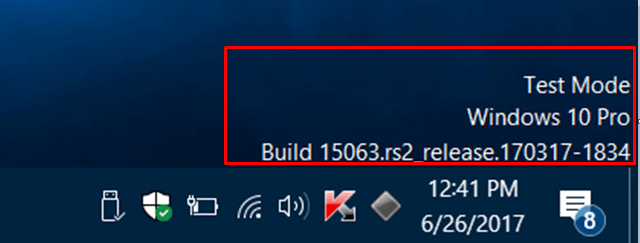
\includegraphics[scale=0.7]{images/testmode.png}
\end{figure}

\subsection[Run LPUS as Administrator]{Run LPUS as Administrator}

LPUS must be run as Administrator because LPUS edits the registry and uses a
special privilege to load the driver. Editing the registry can only be done if
the application is running as an Administrator. If the registry is already set,
LPUS can be run by a user having a special privilege, \texttt{SeLoadDriver}.
However, for convenience, LPUS should be run as an Administrator.
